\documentclass[letter,11pt]{article}
\usepackage[utf8]{inputenc}
\usepackage[T1]{fontenc}
% These are the document margines
\usepackage[left=1.44in, right=1.63in, top=1in, bottom=1in]{geometry}
\usepackage{amsmath}
\usepackage{xfrac}
\usepackage{setspace}
% \usepackage{times}
\usepackage{url}
\usepackage{tikz}
\usepackage{color}
\usepackage{graphics}
\usepackage{float}
\usepackage{verbatim}
\usepackage{listings}
\usepackage{alltt}
\usepackage{algorithm2e}
\SetAlgoLined
\SetKwProg{MyStruct}{Sztruct}{ contains}{end}

\setstretch{1.1}          % Linespacing
\newcounter{myseccnt}     % Section counter
\newcounter{mysubseccnt}  % subsection counter

\newcommand{\mysection}[1]
{\vspace{9mm}\noindent\fontsize{13pt}{15pt}\setcounter{mysubseccnt}{0}
\stepcounter{myseccnt}\textbf{\arabic{myseccnt}. #1}\normalsize\vspace{5mm}}

\newcommand{\mysubsection}[1]
{\vspace{0mm}\noindent\fontsize{13pt}{15pt}\color{black!50}
\stepcounter{mysubseccnt}\textbf{\arabic{myseccnt}.\arabic{mysubseccnt} #1}\normalsize\vspace{5mm}\color{black}}

\newcommand{\dispcode}[1]
{\color{black!60}\fontsize{9pt}{11pt}\selectfont
\texttt{#1}
\color{black}\normalsize}

% This is first line paragraph indent value
\setlength{\parindent}{12mm}
\makeatletter
\renewcommand\@biblabel[1]{#1.}
\makeatother
\newcommand{\mygrey}[1]{\color{black!60}\small\texttt{#1}\normalsize\color{black}\,}

\begin{document}

% This is the paper title
\begin{center}
 \fontsize{21pt}{24pt}\selectfont Tendermint: Consensus without Mining
\end{center}
\vspace{1mm}  

% This is the author name address and etc
\begin{center}
Jae Kwon\\
yk239@cornell.edu\\
Draft v.0.6
\end{center}\vspace{1mm}

% Paper abstract
\begin{center}
 \fontsize{10pt}{12pt}\selectfont
 \parbox{0.8\textwidth}{\textbf{Abstract.} Cryptocurrencies such as Bitcoin enable users to submit payment transactions without going through a centralized trusted organization.  Bitcoin relies on proof-of-work mining to secure consensus which is problematic;  mining requires a massive expenditure of energy, confirmation of transactions is slow, and security is difficult to quantify.  We propose a solution to the blockchain consensus problem that does not require mining by adapting an existing solution to the Byzantine Generals Problem.}
\end{center}


\begin{algorithm}[H]
\MyStruct{Node}{
  Node* parent\;
  int size\;
  \tcp{other stuff}
}
\end{algorithm}


\mysection{Introduction}

Cryptocurrencies have come into the spotlight since the introduction of Bitcoin \cite{conf:nakamoto}.  The objective of cryptocurrency protocols such as Bitcoin is to maintain a live decentralized transaction ledger while defending against double-spend attacks from malicious Byzantine actors that deviate from the protocol.  Consensus of the Bitcoin transaction ledger is secured by a network of miners who compete for rewards in the blockchain.  This mining, or \textit{proof-of-work}, comes with a hefty cost. At today’s Bitcoin prices and reward schedule, miners are rewarded on the order of \$1,500,000 a day to secure the blockchain – and a significant portion of that money is spent on electricity.  Proof-of-work based consensus protocols are also slow, requiring up to an hour to reasonably confirm a payment to prevent double-spending.\\

Alternative protocols have been proposed by the cryptocurrency community to replace proof-of-work mining \cite{conf:nxt, conf:bitshares}.  Some of these protocols suffer from the \textit{nothing at stake problem};  participants have nothing to lose by contributing to multiple blockchain forks, so consensus on a single blockchain is not guaranteed.  Other protocols require participant to accurately gauge the trustworthiness of other key participants, which makes analysis of security difficult to quantify.\\

Our contribution is a novel consensus protocol that requires no proof-of-work mining and has a high level of protection against double-spend attacks.  We make a weak assumption about the participant’s abilities to keep time, and we assume partial synchrony of the network.  Our algorithm is based on a modified version of the DLS protocol \cite{article:dwork}, and is resilient up to $\sfrac{1}{3}$ of Byzantine participants.



\mysection{The Difficulty of Quantifying Security}

Security analysis of cryptocurrency protocols is complicated by many factors.   One such complicating factor is the rational self-interested nature of participants.  The ideal protocol is an incentive compatible Nash equilibrium such that deviating from the protocol does not result in a net gain \cite{article:kroll}.  Recent work by Eyal and Sirer \cite{article:eyal} showed that the Bitcoin protocol is susceptible to a minority collusion group that can grow to become a centralized majority.  They propose a modification to the Bitcoin protocol such that it can tolerate colluding groups that control up to $\sfrac{1}{4}$ of the mining power – less than the previously assumed bound of $\sfrac{1}{2}$ of Byzantine mining power which requires an honest mining majority that follows the prescribed protocol.\\

Another complicating factor is whether the power to achieve or disrupt consensus is extrinsic in origin (e.g. access to the production of mining equipment or access to cheap electricity) or intrinsic in origin (e.g. the “stake” of validators in \textit{proof-of-stake} protocols) and whether the disruption of consensus – especially via a successful double-spend attack – is associated with a commensurate penalty.  The problem with extrinsic factors of security is that they are not easily quantifiable for analysis.  For example, the depreciation costs of Bitcoin mining hardware in the event of a successful double-spend attack may not be significant compared to the running costs of electricity.  On the other hand existing proof-of-stake protocols do not have a well defined intrinsic penalty for instigators of a double-spend attack.  This is commonly called, ironically, the “nothing at stake” problem.  Newer protocols like the BitShares \textit{delegated-proof-of-stake} protocol attempt to address this problem by placing the role of ranked-delegate at stake \cite{conf:bitshares}, but security is dependant  on the extrinsic ability of stakeholders to accurately predict the future performance of delegates.\\

Security analysis is much simpler for an intrinsically secure cryptocurrency protocol when it can be proved that launching a double-spend attack necessarily results in a very high intrinsic penalty compared to the possible intrinsic gains.  Then, the protocol may be considered resistant to double-spent attacks assuming no further extrinsic complications.



\mysection{Terms}

\textit{Nodes} are connected to each other in a peer-to-peer network and relay new information by \textit{gossip}. Each node keeps a complete copy of a totally ordered sequence of events in the form of a \textit{blockchain} as in Bitcoin. \textit{Users} keep an \textit{account} in the system, where the user’s account is identified by the user’s public key or \textit{address}.  Each account can hold a sum of \textit{coins} that can change with new \textit{transactions}. Nodes relay new transactions as they are signed and submitted by users to a node of the network.  A transaction is \textit{valid} if it follows the rules of our protocol (e.g. sufficient funds to send, etc).


\mysection{Block Structure}

Valid transactions are grouped into \textit{blocks} with a structure shown in figure~\ref{fig:block}.  The \textit{validation} and \textit{transactions} hashes are merkle tree root hashes of the signatures and transaction data included in the block \cite{article:merkle}.  The \textit{state hash}, included in the header, is likewise the merkle root hash of the persistent account state (external to the blockchain) after applying the transactions of the block.    Finally the \textit{block hash} is computed by hashing the header, validation, and transactions hashes.  This way, the block hash itself is a merkle root hash such that any component of the block and account state can be verified with a merkle hash trail that leads to the block hash.  A block is said to be valid if all the transactions in the block are valid and sufficient signatures are included in the validation.

\begin{figure}[H]
 \centering
 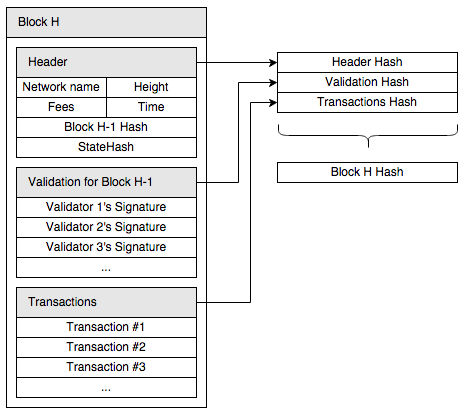
\includegraphics[scale=0.5]{figures/block.png}
 \caption{Block structure}
 \label{fig:block}
\end{figure}


\mysection{Validators}

\textit{Validators} are users with accounts that have coins locked in a bond deposit by posting a \textit{bond transaction}.  These validators participate in the consensus protocol by broadcasting cryptographic signatures, or \textit{votes}, to agree upon the next block.  We say that a validator has \textit{voting power} equal to the amount of the bonded coins.  The validator can later unlock its coins by posting an \textit{unbonding transaction}.  Afterwards the coins remain locked for a predetermined period of time called the \textit{unbonding period}, after which the validator is free to transfer or spend those coins to other accounts.  A set of validators with at least $\sfrac{2}{3}$ of total voting power is also called a \textit{$\sfrac{2}{3}$ majority of validators}.  Similarly, a set of validators with at least $\sfrac{1}{3}$ of total voting power is called a \textit{$\sfrac{1}{3}$ majority of validators}.\\

A block is considered \textit{committed} when a $\sfrac{2}{3}$ majority of validators sign commit votes for that block.  A \textit{fork} occurs when two blocks at the same height are each signed by a $\sfrac{2}{3}$ majority of validators.  By simple arithmetic, a fork can only happen when at least a $\sfrac{1}{3}$ majority of validators signs \textit{duplicitously}.\\

When a validator signs duplicitously, a short \textit{evidence transaction} can be generated by anyone with the two conflicting commit-vote signatures.  This evidence is committed into the blockchain which destroys the bonded coins of the guilty validator(s).  As long as the evidence is committed before the guilty validator’s coins are spent (that is, before the unbonding period is over), the validator can be duly punished.  Note that this does not preclude a $\sfrac{2}{3}$ majority of validators from publishing a blockchain fork after they had unbonded and sold their coins to an unsuspecting party.  This is called a \textit{long-range double-spend attack}.  A user can avoid long-range attacks by syncing their blockchain periodically within the bounds of the unbonding period.\\

A double-spend attack implies a fork in the blockchain.  A \textit{short-range double-spend attack} occurs when a fork happens at a recent height:  recent enough that the guilty validators still have their coins locked in bond.  Since a fork requires at least a $\sfrac{1}{3}$ majority of validators to have signed duplicitously, the penalty for a short-range double-spend attack is a significant proportion ($\sfrac{1}{3}$) of the total amount of bonded coins.  Thus we can adjust the minimum cost of launching a double-spend attack by tuning the incentive to become a validator.  For example, the cryptocurrency can be inflationary by way of block rewards divided amongst the validators in proportion to their voting power.  The inflation rate need not be fixed, but can depend on the past average weighted transaction volume of the network as measured by coin-days-destroyed \cite{conf:daysdestroyed}.  If the marginal cost of securing a validator node is negligible, the reward scheme need not be inflationary;  the transaction fees paid by users may be sufficient.



\mysection{Consensus}

\mysubsection{On Byzantine Consensus}

Fischer et al have shown in a seminal paper \cite{article:fischer} that in an asynchronous system (where no assumptions are made about time) of deterministic processes, no protocol can guarantee consensus even with one faulty process.  This is called the FLP impossibility result.  Much research has gone into understanding ways to circumvent the FLP impossibility result by slightly modifying the problem domain, e.g. by sacrificing determinism, adding time, adding oracles etc \cite{article:correia}.  Bitcoin circumvents the FLP impossibility result by making some assumptions about the synchrony of the network (i.e. nodes soon sync up with the network) and time (i.e. miners dedicate limited time and resources to the best blockchain).\\

Our algorithm is based on algorithm 2’ from section 4 of \cite{article:dwork} (Dwork et al).  It assumes that the network is partially synchronous; there is assumed to be some unknown upper bound $\Delta$ on the time of messages to be delivered.  Intuitively, there may be arbitrary but finite latency in the network.  We also assume that all non-byzantine nodes have access to an internal clock that can stay sufficiently accurate for a short duration of time until consensus on the next block is achieved.  The clocks do not need to agree on a global time and may drift at some bounded rate relative to global time.  The algorithm is adapted to work with blockchains on a gossip network.  As in the algorithm proposed by Dwork et al, it can tolerate of up to $\sfrac{1}{3}$  byzantine voting power.\\



\mysubsection{Algorithm}

validators participate in the consensus process by signing votes for blocks.  There are three types of votes: a \textit{prevote}, a \textit{precommit} and a \textit{commit}.  To \textit{receive more than $\sfrac{2}{3}$ of commits} means to receive commits from a $\sfrac{2}{3}$ majority of validators.  A block is said to be \textit{committed by the network} when a $\sfrac{2}{3}$ majority of validators had signed and broadcast commits for that block.

\begin{figure}[H]
 \centering
 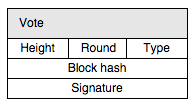
\includegraphics[scale=0.5]{figures/vote.png}
 \caption{Vote structure}
\end{figure}

At each height of the blockchain a round-based protocol is run to determine the next block.  Each round is composed of three steps ($Propose$, $Prevote$, and $Precommit$), along with two special steps $Commit$ and $NewHeight$.  The $Propose$, $Prevote$, and $Precommit$ steps each take one third of the total time allocated for that round.  Each round is longer than the previous round by a small fixed increment of time.  This allows the network to eventually achieve consensus in a partially synchronous network.

\begin{figure}[H]
 \centering
 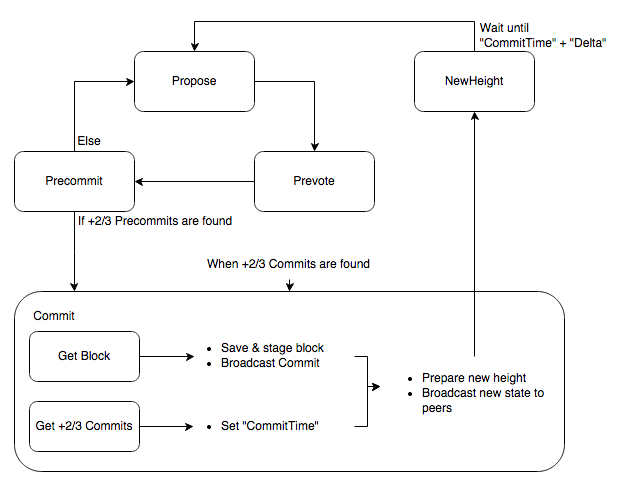
\includegraphics[scale=0.5]{figures/statemachine.png}
 \caption{Overview of state machine}
\end{figure}

Each round has a designated \textit{proposer} chosen in round-robin fashion such that validators are chosen with frequency in proportion to their voting power [TODO: add algorithm to appendix].  Given a blockchain of height $H$ and a deterministic round-robin algorithm, it is clear that all nodes will agree upon the the sequence of proposers for all rounds.

\begin{figure}[H]
 \centering
 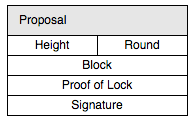
\includegraphics[scale=0.5]{figures/proposal.png}
 \caption{Proposal structure}
\end{figure}

The first step is the $Propose$ step.  In the beginning of the $Propose$ step the designated proposer for that round broadcasts a proposal to its peers via gossip.  If the proposer is locked on a block from some prior round it proposes the locked block and includes a \textit{proof-of-lock} in the proposal (more on that later).  During the $Propose$ step all nodes gossip the proposal to their neighboring peers.\\

In the beginning of the $Prevote$ step each validator makes a decision.  If the validator is locked on a proposed block from some prior round, it signs and broadcasts a prevote for the locked block.  Otherwise if the validator had received an acceptable proposal for the current round, then it signs and broadcasts a prevote for the proposed block.  If the validator had received no proposal or an invalid one, it signs a special $nil$ prevote.  No locking happens during the $Prevote$ step.  During the $Prevote$ step all nodes gossip all prevotes for the round to their neighboring peers.\\

In the beginning of the $Precommit$ step each validator makes a decision.  If the validator had received more than $\sfrac{2}{3}$ of prevotes for a particular acceptable block then the validator signs and broadcasts a precommit for that block.  It also locks onto that block and releases any prior locks.  A node has a lock on at most one block at a time.  If the node had received more than $\sfrac{2}{3}$ of $nil$ prevotes then it simply unlocks.  When locking (or unlocking) the node gathers the prevotes for the locked block (or the prevotes for $nil$) and packages them into a \textit{proof-of-lock} for later when it is its turn to propose.  If a node had not received more than $\sfrac{2}{3}$ of prevotes for a particular block (or $nil$), then it does not sign or lock anything.  During the $Precommit$ step all nodes gossip all precommits for the round to all neighboring peers.\\

At the end of the $Precommit$ step each node makes a decision.  If the node had received more than $\sfrac{2}{3}$ of precommits for a particular block, then the node enters the $Commit$ step.  Otherwise it continues onto the $Propose$ step of the next round.  Even if a node hadn’t yet received the block precommitted by the network, it enters the $Commit$ step.\\

The $Commit$ step is a special step.  There are two parallel conditions that must both be satisfied before finalizing the round.  First, the node must receive the block committed by the network if it hadn’t already.  Once the block is received by a validator it signs and broadcasts a commit for that block.  Second, the node must wait until it receive at least $\sfrac{2}{3}$ of commits for the block precommitted by the network.  Once both conditions are satisfied the node sets its $CommitTime$ to the current time and transitions to the $NewHeight$ step.  The asynchronous and local nature of $CommitTime$ allows the network to maintain consensus despite drifting clocks, as long as the clocks remain accurate enough during the consensus process of a given height.\\

Before the first round (round 0) at height $H$ is the $NewHeight$ step whose purpose is to gather additional commits for the previously committed block at height \textit{H-1}.  Nodes stay at this step until some fixed duration of time past \textit{CommitTime}.  This allows block proposals to include more than the minimum $\sfrac{2}{3}$ of commits, thus allowing the commits of slower validators to be included in the blockchain.\\

At any time during the consensus process if a node receives more than $\sfrac{2}{3}$ of commits for a particular block, it immediately enters the $Commit$ step if it hadn’t already.  Thus there are two ways to enter the $Commit$ step.  A commit-vote for a block at round $R$ counts as prevotes and precommits for all rounds $R’$ where $R < R’$.  Commit-votes are gossipped to neighboring peers in the background regardless of the current round or step.  \\

At any time during the consensus process if a node is locked on a block from round $R$ but receives a \textit{proof-of-lock} for a round $R’$ where $R < R’$, the node unlocks.\\


\mysubsection{Proof of Safety}

If there are less than $\sfrac{1}{3}$ in Byzantine voting power and at least one good validator decides on a block $B$, then no good validator will decide on any block other than $B$.  Consider the earliest round $R$ where at least one good validator commits block $B$ at round $R$.  This validator received more than $\sfrac{2}{3}$ of precommits for block $B$ at round $R$.  Considering that less than $\sfrac{1}{3}$ are Byzantine, by arithmetic at least $\sfrac{1}{3}$ of good validators must have precommitted block $B$ at round $R$.  These good validators must have a lock on block $B$ at round $R$.  No other block can be committed by good validators unless some of the good validators unlock from $B$, which is impossible.\\


\mysubsection{Proof of Liveness}

If there are less than $\sfrac{1}{3}$ in Byzantine voting power then this protocol does not deadlock.  The only way the consensus process can deadlock is if two different blocks had been locked by some good validators from different rounds (a rare occurrence without an active global adversary).  Say that some good validators locked on block $B$ and round $R$, and some good validators locked on block $B’$ at round $R’$, where $R < R’$.  In this case the proof-of-lock from $R’$ included in a proposal by a good validator will eventually unlock those validators locked on $R$ allowing the consensus process to continue.\\


\mysubsection{Cooperation}

Since validators divide the transaction fees of block $H$ amongst themselves, a greedy validator might be tempted to exclude some signatures when proposing the next block \textit{H+1}.  This is an inferior strategy when considering that other validators are game optimal participants.  Given that the total amount of fees to be divided in a block is $f_1$, and that the sum of the voting powers $v_i$ of all validators that have signed and successfully broadcasted their signatures is 1, consider proposer $P$ with voting power $v_p < 1$ who is considering whether to include validator Alice’s signature with voting power $v_a < 1$.  At stake is Alice’s fair share of the fees which is $f_1 \cdot v_a$.  Of this, $P$’s incremental benefit of excluding Alice’s signature is:

\begin{equation*}
 f_1 \cdot v_a \cdot v_p / (1 - v_a)
\end{equation*}

Then, \textit{Alice} could react tit-for-tat by excluding $P$’s signature when it becomes \textit{Alice}’s turn to propose the next block, where the sum of the fees in that block is $f_2$.  In that case, $P$’s detriment is:

\begin{equation*}
 f_2 \cdot v_p
\end{equation*}

$P$ only gains a monetary advantage if the benefit outweighs the costs where:

\begin{equation*}
 f_1 \cdot v_a \cdot v_p / (1 - v_a)  >  f_2 \cdot v_p
\end{equation*}
\begin{equation*}
f_1  >  f_2  / (v_a / (1 - v_a))
\end{equation*}


Thus if $P$ and \textit{Alice}’s interactions were limited such that they only get to propose one block each, it’s clear that $P$ doesn’t benefit overall unless the proposed block contains a much larger sum of fees $f_1$ in reward than what \textit{Alice}’s later block will contain, $f_2$, assuming $v_a \ll 1$.  Even if \textit{Alice}’s voting power is large, she could divide her stake amongst multiple smaller accounts. In the case where $P$ and \textit{Alice} aren’t limited to propose one block each, $P$ and \textit{Alice} might exclude each other’s signatures indefinitely.  In this case, $P$’s expected benefit on each block is:

\begin{equation*}
E[fees] \cdot v_a \cdot v_p \cdot v_p
\end{equation*}

whereas P’s expected detriment on each block is:

\begin{equation*}
E[fees] \cdot v_p \cdot v_a
\end{equation*}

No matter the amount of voting power, no two validators benefit by excluding each other’s signatures indefinitely.  Intuitively, this is because the other validators gain more when two validators exclude each other.



\mysection{Optimizations}

\mysubsection{Sparse Signature Set}

While the protocol described so far is theoretically feasible, in practice there are computational, storage, and network limitations to consider.  We want to allow for as many validator nodes as possible, but it may be too costly to store every validator’s signature for every block.\\

TODO: Describe sparse signature set as DMMV\\


\mysubsection{Handling Validator timeouts}

The network should adapt to validator churn as they go offline for various reasons.  Validators that haven't signed for Y blocks in a row (where $1 \le Y \ll \textit{unbonding-period}$) are considered to have timed-out and are \textit{implicitly unbonded}.  As long as validators churn in a staggered fashion, the active validator set can adjust to account for a changing set of participants.  Validators that need to go offline temporarily might be incentivized to sign an \textit{explicit unbonding transaction} as opposed to timing out, as that allows the active validator set to adjust immediately.  For example, timeouts could result in a some small penalty fee in proportion to the amount of bonded coins, or validators may need to participate for some number of blocks before earning any fees.  Later, (both explicitly and implicitly) unbonded validators can become active once again by submitting another bond transaction before the unbonding period is over.\\


\mysubsection{Faster Block Propagation}

TODO: Describe lib-swift used for broadcasting blocks\\


\mysection{Conclusion}

Tendermint is awesome.  The future is now.\\


\bibliography{bibtex/IEEEabrv.bib,bibtex/references.bib}{}
\bibliographystyle{IEEEtran}
\end{document}



